\subsection{Multi-scale structure of heart valves}

    To fully understand the functional properties of heart valves, multi-scale approaches are needed (Fig. \ref{fig:multiscalevalve}) \cite{salma_heart_2016}. This complex hierarchical structure is what lends to seamless heart valve performance under highly dynamic loading conditions. Heart valves have evolved to have multi-layered leaflet structures. The aortic valve, for example, consists of three histologically distinct layers, whereas the mitral valve has four (Fig. \ref{fig:valvelayers}). The fibrosa layer, which is located on the ventricular side of atrioventricular valves and the atrial side of semilunar valves, is composed of circumferentially aligned collagen fibers that provide the leaflets with the necessary tensile strength to open and transmit forces during coaptation while closed. The spongiosa layer is situated adjacent to the fibrosa and though it contains some collagen, its main constituents are the hydrophilic glycosaminoglycans and proteoglycans, which give the valve its compressive properties and allow it to absorb high forces during coaptation. The ventricularis and atrialis are the layers that are adjacent to blood flow in atrioventricular valvesand semilunar valves, respectively. These layers are rich in radially oriented elastin fibers and facilitate the closure movement by extending the valve leaflet as it opens and recoils when it closes. The annulus and chordae tendineae of the atrioventricular valves and the connection between the leaflets and the surrounding myocardium in the semilunar valves provide additional support. 


    Each layer contains varying amounts of collagen, glycosaminoglycan (GAG), and elastin \cite{carruthers_gene_2012}. The fibrosa layer, facing the outflow surface, consists primarily of a dense network of highly aligned type 1 collagen fibers and contributes to about 45\% of the valve thickness. The central spongiosa layer, approximately 30\% of the leaflet thickness is rich in glycosaminoglycans and water \cite{carruthers_gene_2012}. The ventricularis layer, the remaining 25\% of the leaflet faces the left ventricle inflow surface and is composed of elastin and disorganized collagen. Taken collectively, the three layers of the AV with their elastin, collagen and glycosaminoglycans constituents comprise the ECM of the valve. In addition to the biomechanical role the ECM plays in valve function, it provides a support structure for the underlying valve cell network. The ECM influences cell behavior by providing a source of ligands for cell surface receptors, which transfer mechanical strains experienced at the tissue level down to the cells and ultimately initiating intracellular signaling pathways \cite{wiltz_extracellular_2013}.


%-------------------	begin FIGURE 	-------------------%
\begin{figure}
\centering
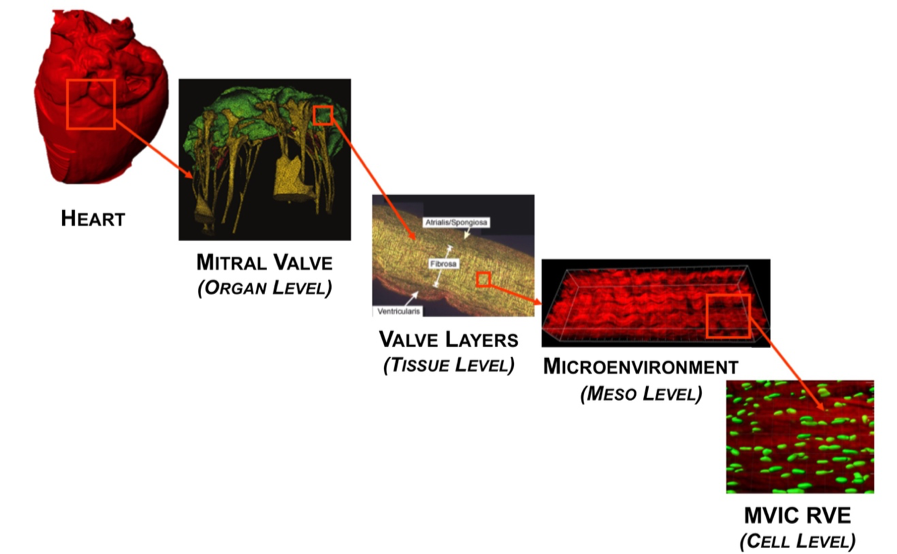
\includegraphics[width=\textwidth]{Images/chapter1/multiscalevalve.png}
\caption{The multiscale nature of heart valve biomechanics: a representation of the mitral valve at the organ-, tissue-, and cell-levels. At the tissue-level: a circumferentially oriented cross-section of the mitral valve anterior leaflet stained with Movat pentachrome, which colors collagen yellow, elastic fibers black, and hydrated PGs and GAGs blue. At the cell-level: a transmission electron micrograph of a mitral VIC from the fibrosa layer. \cite{salma_heart_2016}}
\label{fig:multiscalevalve}
\end{figure}
%-------------------	 end FIGURE 	-------------------%


%-------------------	begin FIGURE 	-------------------%
\begin{figure}
\centering
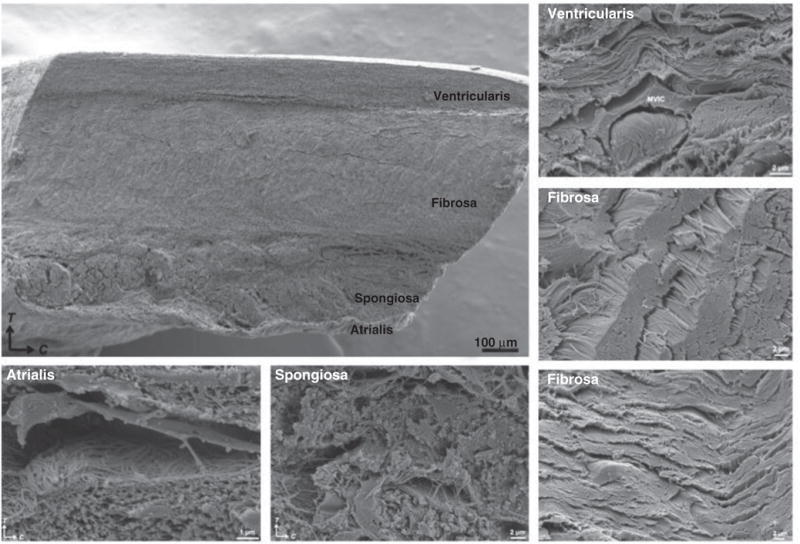
\includegraphics[width=\textwidth]{Images/chapter1/valvelayers.jpg}
\caption{Scanning electron micrograph of the multilayered microenvironment of the MV anterior leaflet. Individual micrographs of each layer are also presented: elastin-rich ventricularis and atrialis, highly collagenous fibrosa, and proteoglycan-rich spongiosa. The collagen fibrils and elastic fibers closely surround the interstitial cells and highlight the long cellular extensions. In the fibrosa, collagen fibrils are aligned in the circumferential direction of the leaflet, which is responsible for the observed anisotropy in leaflet mechanical behavior. (T: transmural, C: circumferential). \cite{salma_heart_2016}}
\label{fig:valvelayers}
\end{figure}
%-------------------	 end FIGURE 	-------------------%




\subsection{Biomechanical function of heart valves}

It has been demonstrated that the individual layers of the aortic valve are not only vastly different in their structure, but also in their mechanical behavior. Two key studies have investigated individual layer behavior of the AV leaflet. Vesely et al. observed the extensibility of intact tissue under uni-axial tension to be significantly different from the individual layer responses [71]. Stella et al. also observed measurably different behaviors under bi-axial loading of separated layers, and reported the intact tissue response to be intermediate to the separated responses [72]. Due to these consistently observed differences in layer behavior, examining the leaflet in an intact state is far more physiologically relevant. 